\begin{figure}
  \centering
  \updatedFigure{
  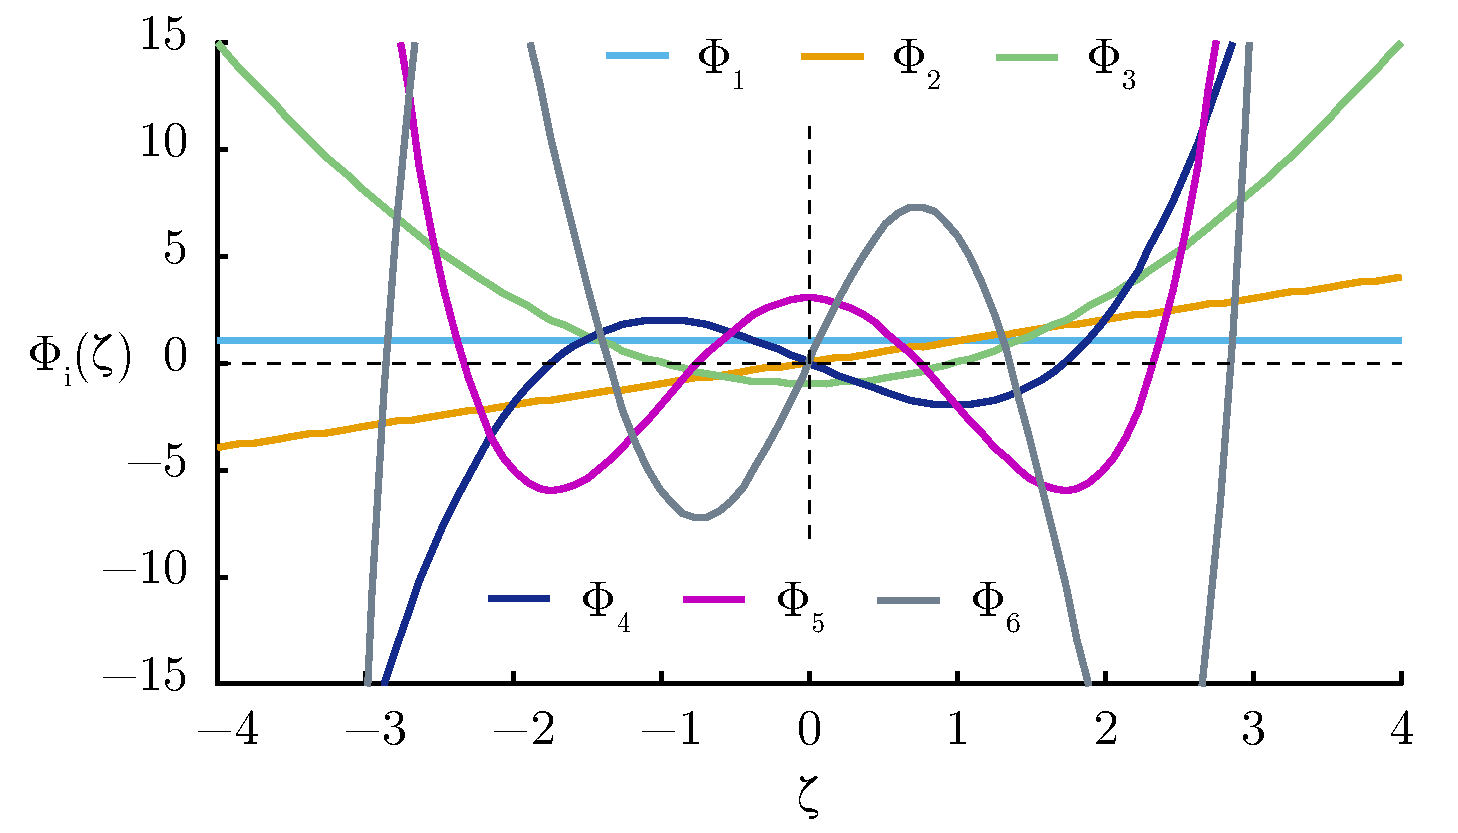
\includegraphics[width=0.9\columnwidth]{include/assets/hermite.pdf}
  }
  \vspace{-1.0em}
  \caption{The first six polynomials of the Hermite basis.}
  \vspace{-1.5em}
  \flabel{hermite}
\end{figure}

\begin{table}[b]
  \vspace{-5pt}
  \centering
  \caption{Probability distributions and polynomial bases.}
  \begin{tabular*}{0.95\linewidth}{llc}
    \toprule
    Distribution & Polynomial basis & Weight function \\
    \midrule
    Gaussian & Hermite & $e^{{-\z^2}/{2}}$ \\
    Uniform & Legendre & $1$ \\
    Beta & Jacobi & $(1 - \z)^\alpha (1 + \z)^\beta$ \\
    Exponential & Laguerre & $e^{-\z}$ \\
    Gamma & Generalized Laguerre & $\z^\alpha e^{-\z}$ \\
    \bottomrule
  \end{tabular*}
  \tlabel{askey}
\end{table}

Due to the inherent complexity, a real-world UQ problem is typically viewed as an approximation problem, wherein one first constructs a light representation of the initial model and then studies the constructed surrogate as it is computationally more efficient; this is the idea behind this paper. The generalized polynomial chaos (PC) \cite{xiu2002} is one way to perform such an approximation, in which the approximating functions are orthogonal polynomials. In this section, we provide some of the basic properties \cite{xiu2010, maitre2010} of this class of polynomials necessary for the PC expansions derived in \sref{polynomial-chaos}.

A set of multivariate polynomials $\{ \pcb_i(\vz) \}$ is orthogonal if
\begin{equation} \elabel{orthogonality}
  \oInner{\pcb_i(\vz)}{\pcb_j(\vz)} = \pcn_i \delta_{ij}, \qquad \forall i, j,
\end{equation}
where $\oInner{\idot}{\idot}$ denotes the inner product in the Hilbert space spanned by the polynomials, $\delta_{ij}$ is the Kronecker delta function, and $\pcn_i = \oInner{\pcb_i(\vz)^2}$ is a normalization constant. The inner product with a weight function $\PDF(\vz)$ is defined as the following multidimensional integral:
\begin{equation} \elabel{inner-product}
  \oInner{f(\vz)}{g(\vz)} = \int f(\vz) g(\vz) \PDF(\vz) d\vz.
\end{equation}
In the stochastic context, $\vz$ is a set of \rvs\ denoted by $\vZ(\o)$, and the weight function corresponds to the \pdf\ of $\vZ(\o)$ (see \sref{uncertain-parameters}). Some of the standard \pdfs\ and the corresponding polynomial bases---which are a part of the Askey scheme \cite{xiu2002} of hypergeometric orthogonal polynomials---are given in \tref{askey}; it can be seen that the weight functions are equal the \pdfs\ up to a constant factor \cite{durrett2010}. Therefore, the inner product coincides with the covariance operator. Consequently, the presence of orthogonality is equivalent to the absence of correlations, and this is what we seek for. Note that, although we focus on continuous \rvs, the generalized PC and, thus, our framework work equally well for discrete probability distributions; see, \eg, \cite{xiu2010, maitre2010, xiu2002}.

The formula of a truncated PC expansion applied to the power term in \eref{recurrence} is given in \sref{polynomial-chaos}, \eref{pc-expansion}. However, we have not shown yet how to find the corresponding coefficients of the expansion, $\pcc{\vP}_{ki}$. To this end, a spectral projection of the stochastic quantity being expanded, \ie, $\vP_k(\o)$, is to be performed onto the space spanned by $\{ \pcb_i(\vZ(\o)) \}_{i = 1}^{\pcterms}$, where $\pcterms$ is the number of polynomials in the truncated basis. This means that one needs to compute inner products of \eref{power-model}, taken at the beginning of the $k$th time interval, with each polynomial from the basis as
\[
  \oInner{\vP_k(\o)}{\pcb_i(\vZ(\o))} = \oInner{\sum_{j=1}^{\pcterms} \pcc{\vP}_{kj} \: \pcb_j(\vZ(\o))}{\pcb_i(\vZ(\o))}
\]
where $i = 1, \dotsc, \pcterms$. Making use of \eref{orthogonality}, we obtain
\begin{equation} \elabel{pc-coefficients}
  \pcc{\vP}_{ki} = \frac{1}{\pcn_i} \oInner{\vP_k(\o)}{\pcb_i(\vZ(\o))}.
\end{equation}
In general, the inner product in \eref{pc-coefficients}, defined by \eref{inner-product}, should be evaluated numerically. This task is independent from the rest of the derivations in this section and, therefore, is discussed in a separate section, \aref{gauss-quadrature}. The total number of the coefficient, $\pcterms$, is given by the following expression, which corresponds to the total-order polynomial space \cite{beck2011}:
\begin{equation} \elabel{pc-terms}
  \pcterms = { \pcorder + \vars \choose \vars } = \frac{(\pcorder + \vars)!}{\pcorder! \vars!}.
\end{equation}
The overall procedure is to be perform for $k = 1, \dotsc, \steps$.

Finally, we need to show the derivation of the recurrent expression in \eref{pc-recurrence}, which is used together with \eref{fourier-output} to compute the PC coefficients of temperature. Using the definition in \eref{pc-expansion}, \eref{expanded-recurrence} can be explicitly written as
\[
  \sum_{i = 1}^{\pcterms} \pcc{\vX}_{ki} \: \pcb_i(\vZ(\o)) = \sum_{i = 1}^{\pcterms} \left( \mCF_k \: \pcc{\vX}_{(k - 1)i} + \mCS_k \: \pcc{\vP}_{ki} \right) \pcb_i(\vZ(\o)).
\]
Multiplying the above equation by each polynomial from the basis and making use of the orthogonality property in \eref{orthogonality}, we obtain \eref{pc-recurrence}. It is worth being mentioned that, since $\vP(\o)$ depends on temperature (see \sref{power-model}), at each step of the iterative process in \eref{pc-recurrence}, the computation of $\pcc{\vP}_{ki}$ should be done with respect to the current PC expansion of temperature, \ie, $\vTO_{k - 1}(\o)$. The computed coefficients can now be utilized to evaluate various statistics of the stochastic power and temperature processes. Moreover, PC series provide analytical expressions for probabilistic moments as shown in \eref{pc-moments}, \sref{output-processing}. Specifically, the formulae in \eref{pc-moments} are due to the fact that, by definition \cite{xiu2010}, the first polynomial $\pcb_1(\vZ(\o))$ in an polynomial basis is unity; hence, $\oExp{\pcb_1(\vZ(\o))} = 1$. Therefore, using \eref{orthogonality}, we conclude that $\oExp{\pcb_i(\vZ(\o))} = 0$ for $i = 2, \dotsc, \pcterms$.

From the development above, it is important to note that the theory of PC expansions suffers from the so-called curse of dimensionality. \eref{pc-coefficients} together with \eref{pc-terms} reveal this major difficulty: when the number of stochastic dimensions increases, the number of polynomial terms as well as the complexity of the corresponding coefficients exhibit a substantial growth, which is exponential without special treatments. The problem does not have a general solution and is one of the central topics of many ongoing studies. In this paper, we mitigate the problem (a) by keeping the number of stochastic dimensions low using the KL expansion as described in \aref{uncertain-parameters} and (b) by using efficient integration techniques as discussed in \aref{gauss-quadrature}.
